\section{Laplace's equation}
    The Laplace equation is a second-order, linear, homogeneous PDE. It is expressed as follows:
    \begin{itemize}
        \item In Cartesian coordinates $(x,y,z)$:
        \begin{align*}
            \laplacian{u}&=\pdv[2]{u}{x}+\pdv[2]{u}{y}+\pdv[2]{u}{z}=0
        \end{align*}

        \item In cylindrical coordinates $(s,\phi,z)$:
        \begin{align*}
            \laplacian{u}&=\dfrac{1}{s}\pdv{s}\qty(s\pdv{u}{s})+\dfrac{1}{s^2}\pdv[2]{u}{\phi}+\pdv[2]{u}{z}=0
        \end{align*}
        \begin{itemize}
            \item \textit{Special case}: In case of azimuthal symmetry, we have $\pdv{u}{\phi}=0$, and so the Laplace equation simplifies to
            \begin{align*}
                \dfrac{1}{s}\pdv{s}\qty(s\pdv{u}{s})+\pdv[2]{u}{z}=0
            \end{align*}
        \end{itemize}

        \item In spherical coordinates $(r,\theta,\phi)$:
        \begin{align*}
            \laplacian{u}&=\dfrac{1}{r^2}\pdv{r}\qty(r^2\pdv{u}{r})+\dfrac{1}{r^2\sin{\theta}}\pdv{\theta}\qty(\sin{\theta}\pdv{u}{\theta})+\dfrac{1}{r^2\sin^2{\theta}}\pdv[2]{u}{\phi}=0
        \end{align*}
        \begin{itemize}
            \item \textit{Special case}: In case of azimuthal symmetry, we have $\pdv{u}{\phi}=0$, and so the Laplace equation simplifies to
            \begin{align*}
                \dfrac{1}{r^2}\pdv{r}\qty(r^2\pdv{u}{r})+\dfrac{1}{r^2\sin{\theta}}\pdv{\theta}\qty(\sin{\theta}\pdv{u}{\theta})=0
            \end{align*}
        \end{itemize}
    \end{itemize}

    \subsection*{Review: spherical coordinate system}
        \begin{figure}[h!]
            \centering
            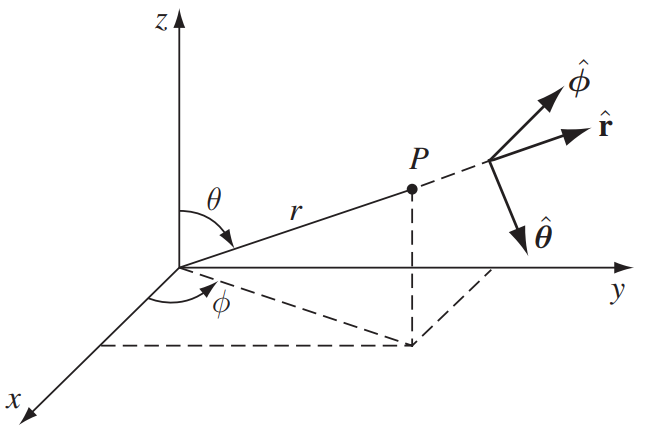
\includegraphics[width=0.5\textwidth]{figures/fig_sph-coor-sys.PNG}
        \end{figure}
        In a spherical coordinate system, any arbitrary point $P$ can be labelled by the spherical coordinates $(r,\theta,\phi)$, where the \textit{radial distance} $r$, \textit{polar angle} $\theta$ and \textit{azimuthal angle} $\phi$ are related to the Cartesian coordinates $(x,y,z)$ as
        \begin{align*}
            x=r\sin{\theta}\cos{\phi},\quad y=r\sin{\theta}\sin{\phi},\quad z=r\cos{\theta}
        \end{align*}
        At any position, the set of orthogonal unit vectors, $\vu{r}$, $\vu{\theta}$ and $\vu{\phi}$, point in the direction of increase of the corresponding coordinates. These unit vectors are related to the Cartesian unit vectors as follows:
        \begin{align*}
            \vu{r}&=\sin{\theta}\cos{\phi}\vu{x}+\sin{\theta}\sin{\phi}\vu{y}+\cos{\theta}\vu{z} \\
            \vu{\theta}&=\cos{\theta}\cos{\phi}\vu{x}+\cos{\theta}\sin{\phi}\vu{y}-\sin{\theta}\vu{z} \\
            \vu{\phi}&=-\sin{\phi}\vu{x}+\cos{\phi}\vu{y}
        \end{align*}
        
        For a given vector $\vb{A}$ if $A_r$, $A_\theta$ and $A_\phi$ represent its radial, polar and azimuthal components, then we have
        \begin{align*}
            \vb{A}=A_r\vu{r}+A_\theta\vu{\theta}+A_\phi\vu{\phi}
        \end{align*}

        The vector derivatives in spherical coordinates are as follows:
        \begin{itemize}
            \item \textit{Gradient}: For a given scalar field $u$, we have
            \begin{align*}
                \grad{u}&=\pdv{u}{r}\vu{r}+\dfrac{1}{r}\pdv{u}{\theta}\vu{\theta}+\dfrac{1}{r\sin{\theta}}\pdv{u}{\phi}\vu{\phi}
            \end{align*}

            \item \textit{Divergence}: For a given vector field $\vb{A}$, we have
            \begin{align*}
                \div{\vb{A}}&=\dfrac{1}{r^2}\pdv{r}\qty(r^2A_r)+\dfrac{1}{r\sin{\theta}}\pdv{\theta}\qty(\sin{\theta}A_\theta)+\dfrac{1}{r\sin{\theta}}\pdv{A_\phi}{\phi}
            \end{align*}

            \item \textit{Curl}: For a given vector field $\vb{A}$, we have
            \begin{align*}
                \curl{\vb{A}}=&\dfrac{1}{r\sin{\theta}}\qty[\pdv{\theta}\qty(\sin{\theta}A_\phi)-\pdv{A_\theta}{\phi}]\vu{r}+\dfrac{1}{r}\qty[\dfrac{1}{\sin{\theta}}\pdv{A_r}{\phi}-\pdv{r}\qty(rA_\phi)]\vu{\phi} \\
                &+\dfrac{1}{r}\qty[\pdv{r}\qty(rA_\theta)-\pdv{A_r}{\theta}]\vu{\phi}
            \end{align*}
        \end{itemize}

    \setcounter{equation}{0}
    \subsection{Laplace's equation in spherical coordinates}
        For any scalar field $u$, its Laplacian is obtained as the divergence of its curl, i.e.
        \begin{align}
            \laplacian{u}=\div{\qty(\grad{u})} \label{eqn:laplacian-div-grad}
        \end{align}

        We know that the gradient of $u$ in spherical coordinates is
        \begin{align}
            \grad{u}&=\pdv{u}{r}\vu{r}+\dfrac{1}{r}\pdv{u}{\theta}\vu{\theta}+\dfrac{1}{r\sin{\theta}}\pdv{u}{\phi}\vu{\phi} \label{eqn:grad-u}
        \end{align}

        Let $\vb{A}$ be a vector field, such that $\vb{A}=\grad{u}$. In terms of its radial, polar and azimuthal components, we can write
        \begin{align}
            \vb{A}&=A_r\vu{r}+A_\theta\vu{\theta}+A_\phi\vu{\phi} \nonumber\\
            \implies\grad{u}&=A_r\vu{r}+A_\theta\vu{\theta}+A_\phi\vu{\phi} \label{eqn:grad-u-A-comp}
        \end{align}
        Comparing equations (\ref{eqn:grad-u}) and (\ref{eqn:grad-u-A-comp}), we obtain
        \begin{align*}
            A_r=\pdv{u}{r},\quad A_\theta=\dfrac{1}{r}\pdv{u}{\theta},\quad A_\phi=\dfrac{1}{r\sin{\theta}}\pdv{u}{\phi}
        \end{align*}

        Now, we know that, the divergence of the vector field $\vb{A}$ in spherical coordinates is
        \begin{align*}
            \div{\vb{A}}&=\dfrac{1}{r^2}\pdv{r}\qty(r^2A_r)+\dfrac{1}{r\sin{\theta}}\pdv{\theta}\qty(\sin{\theta}A_\theta)+\dfrac{1}{r\sin{\theta}}\pdv{A_\phi}{\phi}
        \end{align*}
        
        Substituting for $A_r$, $A_\theta$ and $A_\phi$ above, we obtain
        \begin{align}
            \div{\qty(\grad{u})}&=\dfrac{1}{r^2}\pdv{r}\qty(r^2\pdv{u}{r})+\dfrac{1}{r\sin{\theta}}\pdv{\theta}\qty(\sin{\theta}\dfrac{1}{r}\pdv{u}{\theta})+\dfrac{1}{r\sin{\theta}}\pdv{\phi}\qty(\dfrac{1}{r\sin{\theta}}\pdv{u}{\phi}) \nonumber\\
            \implies\laplacian{u}&=\dfrac{1}{r^2}\pdv{r}\qty(r^2\pdv{u}{r})+\dfrac{1}{r^2\sin{\theta}}\pdv{\theta}\qty(\sin{\theta}\pdv{u}{\theta})+\dfrac{1}{r^2\sin^2{\theta}}\pdv[2]{u}{\phi} \label{eqn:laplacian-sph}
        \end{align}

        Using equation (\ref{eqn:laplacian-sph}), we finally obtain the Laplace's equation in spherical coordinates as
        \begin{align*}
            \laplacian{u}&=0 \\
            \implies\Aboxed{\dfrac{1}{r^2}\pdv{r}\qty(r^2\pdv{u}{r})+\dfrac{1}{r^2\sin{\theta}}&\pdv{\theta}\qty(\sin{\theta}\pdv{u}{\theta})+\dfrac{1}{r^2\sin^2{\theta}}\pdv[2]{u}{\phi}=0}
        \end{align*}

        An alternative form of the Laplace's equation in spherical coordinates is obtained by applying the product rule to the first term. This form is more convenient in certain boundary value problems
        \begin{align*}
            \Aboxed{\pdv[2]{u}{r}+\dfrac{2}{r}\pdv{u}{r}+\dfrac{1}{r^2\sin{\theta}}\pdv{\theta}\qty(\sin{\theta}\pdv{u}{\theta})+\dfrac{1}{r^2\sin^2{\theta}}\pdv[2]{u}{\phi}=0}
        \end{align*}

    \subsection*{Review: cylindrical coordinate system}
        \begin{figure}[h!]
            \centering
            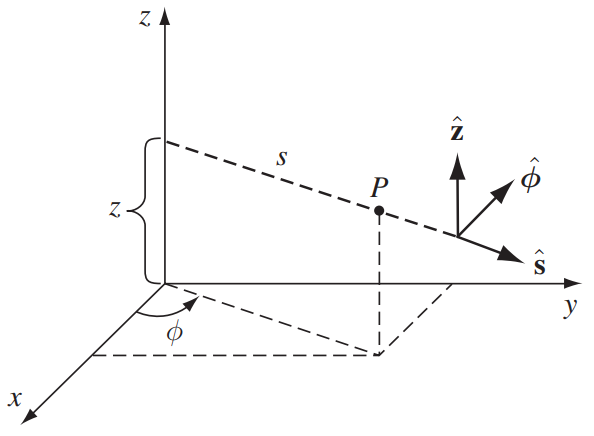
\includegraphics[width=0.5\textwidth]{figures/fig_cyl-coor-sys.PNG}
        \end{figure}
        In a cylindrical coordinate system, any arbitrary point $P$ can be labelled by the cylindrical coordinates $(s,\phi,z)$, where the \textit{axial distance} $s$, \textit{azimuthal angle} $\phi$ and \textit{height} $z$ are related to the Cartesian coordinates $(x,y,z)$ as
        \begin{align*}
            x=s\cos{\phi},\quad y=s\sin{\phi},\quad z=z
        \end{align*}
        At any position, the set of orthogonal unit vectors, $\vu{s}$, $\vu{\phi}$ and $\vu{z}$, point in the direction of increase of the corresponding coordinates. These unit vectors are related to the Cartesian unit vectors as follows:
        \begin{align*}
            \vu{s}&=\cos{\phi}\vu{x}+\sin{\phi}\vu{y} \\
            \vu{\phi}&=-\sin{\phi}\vu{x}+\cos{\phi}\vu{y} \\
            \vu{z}&=\vu{z}
        \end{align*}
        
        For a given vector $\vb{A}$ if $A_s$, $A_\phi$ and $A_z$ represent its axial, azimuthal and height components, then we have
        \begin{align*}
            \vb{A}=A_s\vu{s}+A_\phi\vu{\phi}+A_z\vu{z}
        \end{align*}

        The vector derivatives in cylindrical coordinates are as follows:
        \begin{itemize}
            \item \textit{Gradient}: For a given scalar field $u$, we have
            \begin{align*}
                \grad{u}&=\pdv{u}{s}\vu{s}+\dfrac{1}{s}\pdv{u}{\phi}\vu{\phi}+\pdv{u}{z}\vu{z}
            \end{align*}

            \item \textit{Divergence}: For a given vector field $\vb{A}$, we have
            \begin{align*}
                \div{\vb{A}}&=\dfrac{1}{s}\pdv{s}\qty(sA_s)+\dfrac{1}{s}\pdv{A_\phi}{\phi}+\pdv{A_z}{z}
            \end{align*}

            \item \textit{Curl}: For a given vector field $\vb{A}$, we have
            \begin{align*}
                \curl{\vb{A}}=&\qty(\dfrac{1}{s}\pdv{A_z}{\phi}-\pdv{A_\phi}{z})\vu{s}+\qty(\pdv{A_s}{z}-\pdv{A_z}{s})\vu{\phi}+\dfrac{1}{s}\qty[\pdv{s}\qty(sA_\phi)-\pdv{A_s}{\phi}]\vu{z}
            \end{align*}
        \end{itemize}

    \setcounter{equation}{0}
    \subsection{Laplace's equation in cylindrical coordinates}
        For any scalar field $u$, its Laplacian is obtained as the divergence of its curl, i.e.
        \begin{align}
            \laplacian{u}=\div{\qty(\grad{u})} \label{eqn:laplacian-div-grad}
        \end{align}

        We know that the gradient of $u$ in cylindrical coordinates is
        \begin{align}
            \grad{u}&=\pdv{u}{s}\vu{s}+\dfrac{1}{s}\pdv{u}{\phi}\vu{\phi}+\pdv{u}{z}\vu{z} \label{eqn:grad-u:cyl}
        \end{align}

        Let $\vb{A}$ be a vector field, such that $\vb{A}=\grad{u}$. In terms of its axial, azimuthal and height components, we can write
        \begin{align}
            \vb{A}&=A_s\vu{s}+A_\phi\vu{\phi}+A_z\vu{z} \nonumber\\
            \implies\grad{u}&=A_s\vu{s}+A_\phi\vu{\phi}+A_z\vu{z} \label{eqn:grad-u-A-comp:cyl}
        \end{align}
        Comparing equations (\ref{eqn:grad-u:cyl}) and (\ref{eqn:grad-u-A-comp:cyl}), we obtain
        \begin{align*}
            A_s=\pdv{u}{s},\quad A_\phi=\dfrac{1}{s}\pdv{u}{\phi},\quad A_z=\pdv{u}{z}
        \end{align*}

        Now, we know that, the divergence of the vector field $\vb{A}$ in cylindrical coordinates is
        \begin{align*}
            \div{\vb{A}}&=\dfrac{1}{s}\pdv{s}\qty(sA_s)+\dfrac{1}{s}\pdv{A_\phi}{\phi}+\pdv{A_z}{z}
        \end{align*}
        
        Substituting for $A_s$, $A_\phi$ and $A_z$ above, we obtain
        \begin{align}
            \div{\qty(\grad{u})}&=\dfrac{1}{s}\pdv{s}\qty(s\pdv{u}{s})+\dfrac{1}{s}\pdv{\phi}\qty(\dfrac{1}{s}\pdv{u}{\phi})+\pdv{z}\qty(\pdv{u}{z}) \nonumber\\
            \implies\laplacian{u}&=\dfrac{1}{s}\pdv{s}\qty(s\pdv{u}{s})+\dfrac{1}{s^2}\pdv[2]{u}{\phi}+\pdv[2]{u}{z} \label{eqn:laplacian-cyl}
        \end{align}

        Using equation (\ref{eqn:laplacian-cyl}), we finally obtain the Laplace's equation in cylindrical coordinates as
        \begin{align*}
            \laplacian{u}&=0 \\
            \implies\Aboxed{\dfrac{1}{s}\pdv{s}\qty(s\pdv{u}{s})+&\dfrac{1}{s^2}\pdv[2]{u}{\phi}+\pdv[2]{u}{z}=0}
        \end{align*}

        An alternative form of the Laplace's equation in cylindrical coordinates is obtained by applying the product rule to the first term. This form is more convenient in certain boundary value problems
        \begin{align*}
            \Aboxed{\pdv[2]{u}{s}+\dfrac{1}{s}\pdv{u}{s}+\dfrac{1}{s^2}\pdv[2]{u}{\phi}+\pdv[2]{u}{z}=0}
        \end{align*}

    \textbf{Note}: It is helpful to remember the general forms of the following second order ODEs:
    \begin{itemize}
        \item The general solution of the ODE $\dv[2]{f}{x}-\lambda^2f=0$ is \textit{exponential} in nature and given as
        $$f(x)=c_1e^{\lambda x}+c_2e^{-\lambda x}$$
        \item The general solution of the ODE $\dv[2]{f}{x}+\lambda^2f=0$ is \textit{harmonic} in nature and given as
        $$f(x)=c_1\cos{\lambda x}+c_2\sin{\lambda x}$$
    \end{itemize}

    \subsection*{Examples}
        \begin{enumerate}
            \setcounter{equation}{0}
            \item Solve the Laplace equation over a rectangle in the $xy$-plane for the unknown function $u(x,y)$ with the following boundary conditions:
            \begin{align*}
                u(x,0)=0&,\;u(x,b)=0 \\
                u(0,y)=0&,\;u(a,y)=f(y).
            \end{align*}
            \textbf{Solution}: The Laplace equation in the $xy$-plane is
            \begin{align}
                \pdv[2]{u}{x}+\pdv[2]{u}{y}=0 \label{eqn:lapl:eg-1:laplacian-2d}
            \end{align}
            We assume a solution of the form:
            \begin{align}
                u(x,y)=X(x)Y(y) \label{eqn:lapl:eg-1:asm-soln}
            \end{align}
            which gives us
            \begin{align*}
                \pdv[2]{u}{x}=Y\dv[2]{X}{x}\qq{and}\pdv[2]{u}{y}=X\dv[2]{Y}{y}.
            \end{align*}
            Then, substituting in equation (\ref{eqn:lapl:eg-1:laplacian-2d}), we have
            \begin{align*}
                Y\dv[2]{X}{x}+X\dv[2]{Y}{y}=0
            \end{align*}
            Dividing the above throughout by $X(x)Y(y)$, we obtain
            \begin{align}
                \dfrac{1}{X}\dv[2]{X}{x}&+\dfrac{1}{Y}\dv[2]{Y}{y}=0 \nonumber\\
                \implies\dfrac{1}{Y}\dv[2]{Y}{y}&=-\dfrac{1}{X}\dv[2]{X}{x} \label{eqn:lapl:eg-1:separated}
            \end{align}
            In equation (\ref{eqn:lapl:eg-1:separated}), the LHS depends only on $y$, while the RHS depends only on $x$. Hence, the only way for this to be satisfied is if both side equal some separation constant.

            \textit{Case I}: the separation constant is positive, i.e.
            \begin{align*}
                \dfrac{1}{Y}\dv[2]{Y}{y}&=-\dfrac{1}{X}\dv[2]{X}{x}=\lambda^2
            \end{align*}
            We separate these into two ODEs as follows:
            \begin{multicols}{2}
            \setlength{\columnseprule}{0.4pt}
                For the function $Y(y)$:
                \begin{align*}
                    \dfrac{1}{Y}\dv[2]{Y}{y}&=\lambda^2 \\
                    \implies\dv[2]{Y}{y}&=\lambda^2Y \\
                    \implies\dv[2]{Y}{y}-\lambda^2Y&=0
                \end{align*}
                The above ODE has the general solution
                \begin{align}
                    Y(y)&=c_1e^{\lambda y}+c_2e^{-\lambda y} \label{eqn:lapl:eg-1:y-gen-soln-1}
                \end{align}
                
                \columnbreak
                For the function $X(x)$:
                \begin{align*}
                    -\dfrac{1}{X}\dv[2]{X}{x}&=\lambda^2 \\
                    \implies\dv[2]{X}{x}&=-\lambda^2X \\
                    \implies\dv[2]{X}{x}+\lambda^2X&=0
                \end{align*}
                The above ODE has the general solution
                \begin{align}
                    X(x)&=c_3\cos{\lambda x}+c_4\sin{\lambda x} \label{eqn:lapl:eg-1:x-gen-soln-1}
                \end{align}
                
            \end{multicols}
            From the boundary condition $u(x,0)=0$, we have that
            \begin{align*}
                X(x)Y(0)&=0 \\
                \implies Y(0)&=0 \\
                \implies c_1e^{0}+c_2e^{0}&=0 \\
                \implies c_2&=-c_1
            \end{align*}
            Again, from the boundary condition $u(x,b)=0$, we have that
            \begin{align*}
                X(x)Y(b)&=0 \\
                \implies Y(b)&=0 \\
                \implies c_1e^{\lambda b}+c_2e^{-\lambda b}&=0 \\
                \implies c_1e^{\lambda b}-c_1e^{-\lambda b}&=0\quad[\because\;c_2=-c_1] \\
                \implies c_1\underbrace{\qty(e^{\lambda b}-e^{-\lambda b})}_{\neq 0}&=0 \\
                \implies c_1&=0\qq{and}c_2=0
            \end{align*}
            This means that $Y(y)=0$, thereby $u(x,y)=0$ everywhere, which is not possible.

            Therefore, this case with a positive separation constant is ruled out.

            \textit{Case II}: the separation constant is negative, i.e.
            \begin{align*}
                \dfrac{1}{Y}\dv[2]{Y}{y}&=-\dfrac{1}{X}\dv[2]{X}{x}=-\lambda^2
            \end{align*}
            We separate these into two ODEs as follows:
            \begin{multicols}{2}
            \setlength{\columnseprule}{0.4pt}
                For the function $Y(y)$:
                \begin{align*}
                    \dfrac{1}{Y}\dv[2]{Y}{y}&=-\lambda^2 \\
                    \implies\dv[2]{Y}{y}&=-\lambda^2Y \\
                    \implies\dv[2]{Y}{y}+\lambda^2Y&=0
                \end{align*}
                The above ODE has the general solution
                \begin{align}
                    Y(y)&=c_5\cos{\lambda y}+c_6\sin{\lambda y} \label{eqn:lapl:eg-1:y-gen-soln-2}
                \end{align}
                
                \columnbreak
                For the function $X(x)$:
                \begin{align*}
                    -\dfrac{1}{X}\dv[2]{X}{x}&=-\lambda^2 \\
                    \implies\dv[2]{X}{x}&=\lambda^2X \\
                    \implies\dv[2]{X}{x}-\lambda^2X&=0
                \end{align*}
                The above ODE has the general solution
                \begin{align}
                    X(x)&=c_7e^{\lambda x}+c_8e^{-\lambda x} \label{eqn:lapl:eg-1:x-gen-soln-2}
                \end{align}
                
            \end{multicols}
            Again, from the boundary condition $u(x,0)=0$, we have that
            \begin{align*}
                Y(0)&=0 \\
                \implies c_5\cos{0}+c_6\sin{0}&=0 \\
                \implies c_5&=0
            \end{align*}
            This gives us
            \begin{align}
                Y(y)&=c_6\sin{\lambda y} \label{eqn:lapl:eg-1:y-gen-soln-3}
            \end{align}
            Applying the boundary condition $u(x,b)=0$ on equation (\ref{eqn:lapl:eg-1:y-gen-soln-3}), we have
            \begin{align*}
                Y(b)=c_6\sin{\lambda b}&=0 \\
                \implies \sin{\lambda b}&=0 \\
                \implies \sin{\lambda b}&=\sin{n\pi} \\
                \implies \lambda b&=n\pi \\
                \implies \lambda&=\dfrac{n\pi}{b}
            \end{align*}
            Then equations (\ref{eqn:lapl:eg-1:x-gen-soln-2}) and (\ref{eqn:lapl:eg-1:y-gen-soln-3}) become
            \begin{align}
                X(x)&=c_7e^{n\pi x/b}+c_8e^{-n\pi x/b} \label{eqn:lapl:eg-1:x-gen-soln-3}\\
                Y(y)&=c_6\sin\qty(\dfrac{n\pi y}{b}) \label{eqn:lapl:eg-1:y-gen-soln-4}
            \end{align}
            Inserting equations (\ref{eqn:lapl:eg-1:x-gen-soln-3}) and (\ref{eqn:lapl:eg-1:y-gen-soln-4}) into equation (\ref{eqn:lapl:eg-1:asm-soln}), we have
            \begin{align}
                u(x,y)&=c_6\sin\qty(\dfrac{n\pi y}{b})\qty[c_7e^{n\pi x/b}+c_8e^{-n\pi x/b}] \label{eqn:lapl:eg-1:gen-u-1}
            \end{align}

            Applying the boundary condition $u(0,y)=0$ on equation (\ref{eqn:lapl:eg-1:gen-u-1}), we have
            \begin{align*}
                u(0,y)&=0 \\
                \implies \underbrace{c_6\sin\qty(\dfrac{n\pi y}{b})}_{\neq 0}\qty[c_7e^{0}+c_8e^{0}]&=0 \\
                \implies c_7+c_8&=0 \\
                \implies c_8&=-c_7
            \end{align*}
            which gives us, from equation (\ref{eqn:lapl:eg-1:gen-u-1}),
            \begin{align}
                u(x,y)&=c_6c_7\sin\qty(\dfrac{n\pi y}{b})\underbrace{\qty[e^{n\pi x/b}-e^{-n\pi x/b}]}_{=2\sinh\qty({n\pi x}/{b})} \nonumber\\
                    &=2c_6c_7\sin\qty(\dfrac{n\pi y}{b})\sinh\qty(\dfrac{n\pi x}{b}) \nonumber\\
                \implies u(x,y)&=C_n\sin\qty(\dfrac{n\pi y}{b})\sinh\qty(\dfrac{n\pi x}{b}) \label{eqn:lapl:eg-1:gen-u-2}
            \end{align}
            where $C_n=2c_6c_7$.

            Finally, applying the last boundary condition $u(a,y)=f(y)$ on equation (\ref{eqn:lapl:eg-1:gen-u-2}), we have
            \begin{align}
                u(a,y)&=f(y) \nonumber\\
                \implies C_n\sin\qty(\dfrac{n\pi y}{b})\sinh\qty(\dfrac{n\pi a}{b})&=f(y) \nonumber\\
                \implies C_n\sin\qty(\dfrac{n\pi y}{b})&=\dfrac{f(y)}{\sinh\qty(\dfrac{n\pi a}{b})} \nonumber\\
                \implies C_n\sin\qty(\dfrac{n\pi y}{b})\times\sin\qty(\dfrac{n\pi y}{b})&=\dfrac{f(y)}{\sinh\qty(\dfrac{n\pi a}{b})}\times\sin\qty(\dfrac{n\pi y}{b}) \nonumber\\
                \implies C_n\sin^2\qty(\dfrac{n\pi y}{b})&=\dfrac{f(y)}{\sinh\qty(\dfrac{n\pi a}{b})}\sin\qty(\dfrac{n\pi y}{b}) \nonumber\\
                \implies C_n\underbrace{\int\limits_{0}^{b}{\sin^2\qty(\dfrac{n\pi y}{b}) \dd{y}}}_{={b}/{2}}&=\dfrac{1}{\sinh\qty(\dfrac{n\pi a}{b})}\int\limits_{0}^{b}{f(y)\sin\qty(\dfrac{n\pi y}{b}) \dd{y}} \nonumber\\
                \implies C_n\times\dfrac{b}{2}&=\dfrac{1}{\sinh\qty(\dfrac{n\pi a}{b})}\int\limits_{0}^{b}{f(y)\sin\qty(\dfrac{n\pi y}{b}) \dd{y}} \nonumber\\
                \implies C_n&=\dfrac{2}{b\sinh\qty(\dfrac{n\pi a}{b})}\int\limits_{0}^{b}{f(y)\sin\qty(\dfrac{n\pi y}{b}) \dd{y}} \label{eqn:lapl:eg-1:Cn}
            \end{align}

            Therefore, the most general solution to the Laplace equation over the given rectangular region is given by
            \begin{align*}
                \Aboxed{u(x,y)&=\sum_{n=1}^{\infty}{C_n\sin\qty(\dfrac{n\pi y}{b})\sinh\qty(\dfrac{n\pi x}{b})}}
            \end{align*}
            where the coefficients, given by equation (\ref{eqn:lapl:eg-1:Cn}), are known from the specified function $f(y)$. 
            
        \end{enumerate}